\documentclass[11pt]{article}

\topmargin -.5in
\textheight 9in
\oddsidemargin -.25in
\evensidemargin -.25in
\textwidth 7in

\usepackage{amsthm}
\usepackage{amssymb, amsmath}
\usepackage{fancyhdr}
\usepackage{enumitem}
\usepackage{tikz}
\usepackage{graphicx}

\usetikzlibrary{trees}

\newcommand{\numpy}{{\tt numpy}}    % tt font for numpy
\newcommand{\floor}[1]{\left\lfloor #1 \right\rfloor}
\newcommand{\ceil}[1]{\left\lceil #1 \right\rceil}

\newtheorem{theorem}{Theorem}[section]
\newtheorem{lemma}[theorem]{Lemma}
\renewcommand\qedsymbol{$\blacksquare$}

\begin{document}

\author{Chunho Lin* (3226964170)\\chunholi@usc.edu}
\title{CSCI-570 Homework 2}
\maketitle

\medskip

\begin{enumerate}

\item \textbf{Problem 1.}

When discussing the implementation of binary heaps we said that the data is stored in an array. Since we did not impose any limits on the size of the heap, it means that we have to use an unbounded array. However, when discussing the runtime of the operations, we did not consider the cost of re-sizing (copying the entries) the array. Show that the cost of \texttt{build} in the online case (i.e. inserting \(n\) entries into an empty heap) is \(O(n \cdot log n)\) even with the cost of copying taken into account. For the sake of simplicity you may assume that we store the root of the heap at index 0, instead of leaving it empty. Provide detailed calculations for the runtime.

\begin{flushright}
[Hint: revisit the cost analysis of unbounded arrays.]
\end{flushright}

\begin{flushright}
\textbf{[4 points]}
\end{flushright}

\begin{proof}[\underline{Proof}]

When we build a binary heap in online case by inserting \(n\) entries into an empty heap, we need to consider two types of costs: the cost of insertions and the cost of expansions the array.

\[
\text{Total Cost } T(n) = \text{Cost of Insertions} + \text{Cost of Expansions}
\]

For the cost of insertion:

\[
\text{Cost of Insertions} = log 1 + log 2 + log 3 + \cdots + log n
\]

For the cost of expansions:

\[
\text{Cost of Expansions} = 2^0 + 2^1 + 2^2 + \cdots + 2^{log n}
\]


Total Cost:

\[
\begin{aligned}
T(n)
&= \bigl(\log 1 + \log 2 + \log 3 + \cdots + \log n \bigr) 
   + \bigl(2^0 + 2^1 + 2^2 + \cdots + 2^{\log n}\bigr) \\[6pt]
&= \sum_{k=1}^{n} \log k \;+\; \sum_{k=0}^{\log n} 2^k \\[6pt]
&= \log(n!) \;+\; \frac{2^{\log n + 1} - 1}{2 - 1} 
   \qquad \text{(geometric series sum)} \\[6pt]
&= \log(n!) \;+\; 2^{\log n + 1} - 1 \\[6pt]
&= \log(n!) \;+\; 2 \cdot 2^{\log n} - 1 \\[6pt]
&= \log(n!) \;+\; 2n - 1. 
\end{aligned}
\]

Using the bound \(\log(n!) < n \log n\), we obtain
\[
T(n) < n \log n + 2n - 1 \;\in\; O(n \log n).
\]

\underline{Conclusion.} The cost of \texttt{build} in the online case is \(O(n \cdot log n)\) even with the cost of copying taken into account.

\end{proof}

% \newpage

\item \textbf{Problem 2.}

Suppose you have two binary min-heaps, \(A\) and \(B\), with a total of \(n\) elements between them. You want to know whether \(A\) and \(B\) have a key in common. Devise an algorithm that solves this problem in \(O(n \cdot log n)\) time and besides the two binary heaps it only uses an array of length 2.

\begin{flushright}
[Hint: first come up with a \(O(n \cdot log n)\) algorithm\\
without the restriction on the size of extra storage.]
\end{flushright}

\begin{flushright}
\textbf{[4 points]}
\end{flushright}

\begin{proof}[\underline{Proof}]

We maintain an auxiliary array of length two: \texttt{arr[0]} will hold the current root of heap \(A\), and \texttt{arr[1]} will hold the current root of heap \(B\).  
The algorithm proceeds as follows:

\begin{enumerate}[label=\arabic*.]
    \item Begin with two nonempty min-heaps \(A\) and \(B\).
    \item At each step, copy the root of heap \(A\) into \texttt{arr[0]} and the root of heap \(B\) into \texttt{arr[1]}.
    \item Compare the two values:
    \begin{itemize}
        \item If they are equal, then a common key has been found, and the algorithm terminates successfully.
        \item If the value in \texttt{arr[0]} is smaller, remove the root of heap \(A\) (i.e., perform \texttt{deleteMin} on \(A\)).
        \item If the value in \texttt{arr[1]} is smaller, remove the root of heap \(B\).
    \end{itemize}
    \item Continue this process until at least one of the heaps becomes empty.
    \item If no equality has been found by the time one heap is exhausted, then no common key exists, and the algorithm returns \texttt{False}.
\end{enumerate}

\underline{Correctness.} 
The algorithm works because both heaps are min-heaps, so the smallest elements are always available at the root. By comparing the roots at each step, we ensure that no potential common key is skipped: if the roots are equal, we have found a common key; if not, the smaller root cannot possibly appear later in the other heap, so it is safely removed. This guarantees that all possible matches are checked.

\underline{Time Complexity.} 
Each comparison and deletion takes \(O(\log n)\) time. In the worst case, we may perform up to \(n\) deletions (when all elements are distinct). Hence, the overall time complexity is \(O(n \log n)\).
\end{proof}


\item \textbf{Problem 3.}

You are given a "k-sorted array": this is an almost-sorted array, where each of the elements are misplaced by less than \(k\) positions from their correct location. For example, \(A = [1, 2, 3, 6, 4, 5, 7]\) is a 3-sorted array, because the elements 4, 5, and 6 are misplaced by 1, 1, and 2 positions respectively from their correct locations. Design an \(O(n \cdot log k)\) algorithm to sort the array and analyze the runtime.

\begin{flushright}
[Hint: using a small heap will be helpful.]
\end{flushright}

\begin{flushright}
\textbf{[5 points]}
\end{flushright}

\begin{proof}[\underline{Proof}]

We are given a \(k\)-sorted array, i.e., each element is at most \(k\) positions away from its correct sorted position. To exploit this property, we use a min-heap with size of \(k+1\):

\begin{enumerate}[label=\arabic*.]
\item Initialize an empty min-heap.
\item Insert the first $k+1$ elements of the array into the heap.
\item For each index $i$ from $0$ to $n-1$:
\begin{enumerate}
\item Perform a \texttt{deleteMin} on the heap. This removes the smallest element from the heap and returns it. Place this value into the output array at position $i$.
\item If there are still elements left in the input array, insert the next element (at index $i+k+1$) into the heap.
\end{enumerate}
\item After all input elements have been considered, repeatedly apply \texttt{deleteMin} on the heap until it becomes empty, appending each result to the output array.
\end{enumerate}

\underline{Correctness.} Because each element is at most $k$ positions from its sorted position, the next smallest element must lie within the current $k+1$ candidates in the heap. The \texttt{deleteMin} operation always returns this globally smallest candidate, ensuring elements are placed in the correct sorted order.

\underline{Time Complexity.}
\begin{itemize}
\item Building the initial heap with $k+1$ elements takes $O(k)$.
\item Each \texttt{deleteMin} and \texttt{insert} operation takes $O(\log k)$.
\item There are $n$ \texttt{deleteMin} operations and at most $n$ \texttt{insert} operations.
\end{itemize}
Thus the total running time is

$$
O(k) + O(n \log k) = O(n \log k).
$$

\end{proof}


\item \textbf{Problem 4.}

Write a divide and conquer algorithm that finds the largest difference between any two elements of an unsorted array of \(n\) numbers.

Example: in case of \(A = [3, 7.65, -2, 3, -0.85, 9.15, -1.5]\)\\
the algorithm should return 11.15.

Your algorithm should run in \(O(n)\) time. To achieve this, the algorithm needs \(T(n) = 2 \cdot T (\frac{n}{2}) + O(1)\) as its runtime recurrence relation. After providing the algorithm, justify that its runtime is indeed \(O(n)\) by unrolling its recursion tree.

\begin{flushright}
\textbf{[5 points]}
\end{flushright}

\begin{proof}[\underline{Proof}]

The divide and conquer algorithm to find the largest difference works as follows:

\begin{enumerate}[label=\arabic*.]
    \item \textbf{Base case:} If the array has only one or two elements, return the difference between the maximum and minimum elements (0 for one element).
    \item \textbf{Divide:} Split the array into two halves.
    \item \textbf{Conquer:} Recursively find:
    \begin{itemize}
        \item The maximum and minimum elements in the left half
        \item The maximum and minimum elements in the right half
    \end{itemize}
    \item \textbf{Combine:} The largest difference is the maximum of:
    \begin{itemize}
        \item The largest difference within the left half
        \item The largest difference within the right half  
        \item The difference between the maximum of both halves and the minimum of both halves
    \end{itemize}
\end{enumerate}

\begin{figure}[h]
\centering
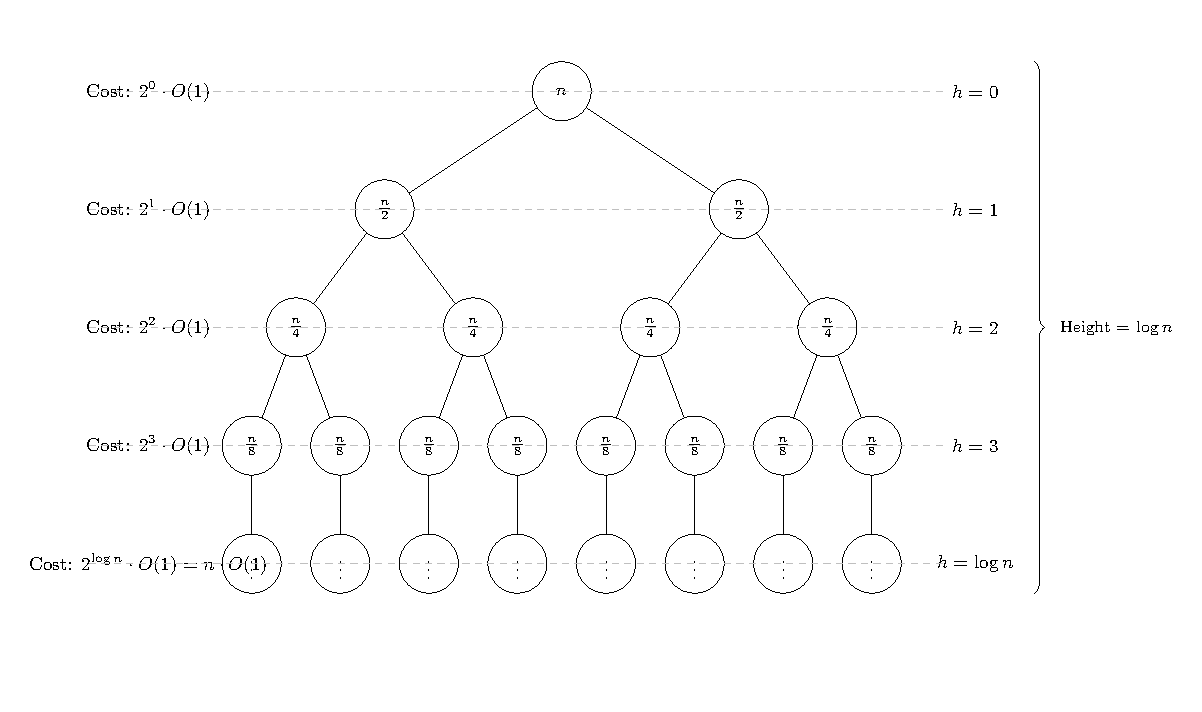
\includegraphics[width=0.75\textwidth]{p4.pdf}
\caption{Recursion tree for the divide and conquer algorithm}
\end{figure}

\newpage

\underline{Recurrence Relation:} $T(n) = 2 \cdot T(\frac{n}{2}) + O(1)$

\underline{Time Complexity:}


From the recursion tree analysis:
\begin{itemize}
    \item \textbf{Height:} $\log n$ levels
    \item \textbf{Cost per level:} Each level has $2^i$ nodes, each doing $O(1)$ work
    \item \textbf{Level 0:} $1 \cdot O(1) = O(1)$
    \item \textbf{Level 1:} $2 \cdot O(1) = O(1)$
    \item \textbf{Level 2:} $4 \cdot O(1) = O(1)$
    \item $\vdots$
    \item \textbf{Level $\log n$:} $2^{\log n} \cdot O(1) = n \cdot O(1) = O(n)$
\end{itemize}

\underline{Total Cost:} 
$$T(n) = \sum_{i=0}^{\log n} 2^i \cdot O(1) = O(1) \cdot \sum_{i=0}^{\log n} 2^i = O(1) \cdot (2^{\log n + 1} - 1) = O(1) \cdot (2n - 1) = O(n)$$

Therefore, the algorithm runs in $O(n)$ time as required.

\end{proof}

\end{enumerate}

\end{document}
